\documentclass[UTF8,zihao=-4]{ctexart}
\usepackage[a4paper,margin=2.5cm]{geometry}
\usepackage{amsmath, amssymb, amsthm}
\usepackage{bm}
\usepackage{hyperref}
\usepackage{graphicx}
\usepackage{caption}
\usepackage{listings}
\usepackage{xcolor}
\usepackage{float}
\usepackage{placeins}
\graphicspath{{figures/}}

% Code style
\lstdefinestyle{code}{
  basicstyle=\ttfamily\small,
  numbers=left,
  numberstyle=\tiny,
  numbersep=8pt,
  keywordstyle=\color{blue},
  commentstyle=\color{teal!70!black},
  stringstyle=\color{orange!70!black},
  showstringspaces=false,
  breaklines=true,
  frame=single,
  framerule=0.3pt,
  rulecolor=\color{black!15}
}
\lstset{style=code}

\title{生成模型:自编码器、对抗网络与扩散模型}
\author{}
\date{\today}

\begin{document}
\maketitle
\tableofcontents
\FloatBarrier

\section{自编码器(AE, VAE)}
自编码器通过重建输入来学习紧凑的潜在表示。编码器 $f_\phi$ 将输入 $\mathbf{x}$ 映射为潜在向量 $\mathbf{z}$,解码器 $g_\theta$ 重建 $\hat{\mathbf{x}}$。图~\ref{fig:autoencoder_architecture_cn} 展示了典型瓶颈结构。

\subsection{确定性自编码器}
最常见的重建损失为均方误差:
\begin{equation}
  \mathcal{L}_{\mathrm{AE}}(\theta, \phi) = \frac{1}{N} \sum_{i=1}^{N} \left\| g_\theta(f_\phi(\mathbf{x}_i)) - \mathbf{x}_i \right\|_2^2.
\end{equation}
基础 AE 容易出现潜在空间不连续,为此可加入正则项:
\begin{itemize}
  \item \textbf{稀疏 AE:} 对激活添加 $L_1$ 正则使潜在表示更稀疏。
  \item \textbf{去噪 AE:} 使用带噪输入 $\tilde{\mathbf{x}}$,重建原始 $\mathbf{x}$,提升鲁棒性。
  \item \textbf{收缩 AE:} 惩罚雅可比 $\|\nabla_{\mathbf{x}} f_\phi(\mathbf{x})\|_F^2$,提升对局部扰动的稳健性。
\end{itemize}

\subsection{变分自编码器}
VAE 引入概率潜变量模型,先验 $p(\mathbf{z}) = \mathcal{N}(\mathbf{0}, \mathbf{I})$,解码分布 $p_\theta(\mathbf{x} \mid \mathbf{z})$。对每个样本的证据下界(ELBO)为
\begin{equation}
  \log p_\theta(\mathbf{x}) \ge \mathbb{E}_{q_\phi(\mathbf{z} \mid \mathbf{x})}[\log p_\theta(\mathbf{x} \mid \mathbf{z})] - \mathrm{KL}(q_\phi(\mathbf{z} \mid \mathbf{x}) \,\|\, p(\mathbf{z})).
\end{equation}
若 $q_\phi(\mathbf{z} \mid \mathbf{x}) = \mathcal{N}\bigl(\boldsymbol{\mu}_\phi(\mathbf{x}), \operatorname{diag}(\boldsymbol{\sigma}^2_\phi(\mathbf{x}))\bigr)$,可使用重参数技巧:
\begin{equation}
  \mathbf{z} = \boldsymbol{\mu}_\phi(\mathbf{x}) + \boldsymbol{\sigma}_\phi(\mathbf{x}) \odot \boldsymbol{\epsilon}, \quad \boldsymbol{\epsilon} \sim \mathcal{N}(\mathbf{0}, \mathbf{I}).
\end{equation}
KL 项的闭式形式为
\begin{equation}
  \mathrm{KL} = -\tfrac{1}{2} \sum_{j=1}^{d} \left(1 + \log \sigma_j^2 - \mu_j^2 - \sigma_j^2 \right).
\end{equation}

\subsection{Beta-VAE 与解耦表示}
$\beta$-VAE 将 KL 项缩放为 $\mathcal{L} = \mathbb{E}[\log p_\theta(\mathbf{x} \mid \mathbf{z})] - \beta\,\mathrm{KL}(q_\phi \| p)$,当 $\beta > 1$ 时可促进潜变量解耦。互信息惩罚、总相关(Total Correlation)约束进一步强化独立性。

\subsection{训练流程}
\begin{lstlisting}[language=Python, caption={带 KL 预热的 VAE 训练循环。}]
for epoch in range(num_epochs):
    beta = min(1.0, epoch / kl_warmup_epochs)
    for x in dataloader:
        mu, logvar = encoder(x)
        z = mu + torch.exp(0.5 * logvar) * torch.randn_like(mu)
        x_recon = decoder(z)
        recon_loss = reconstruction_criterion(x_recon, x)
        kl = -0.5 * (1 + logvar - mu.pow(2) - logvar.exp()).sum(dim=1).mean()
        loss = recon_loss + beta * kl
        loss.backward()
        optimizer.step()
        optimizer.zero_grad()
\end{lstlisting}

\begin{figure}[H]
  \centering
  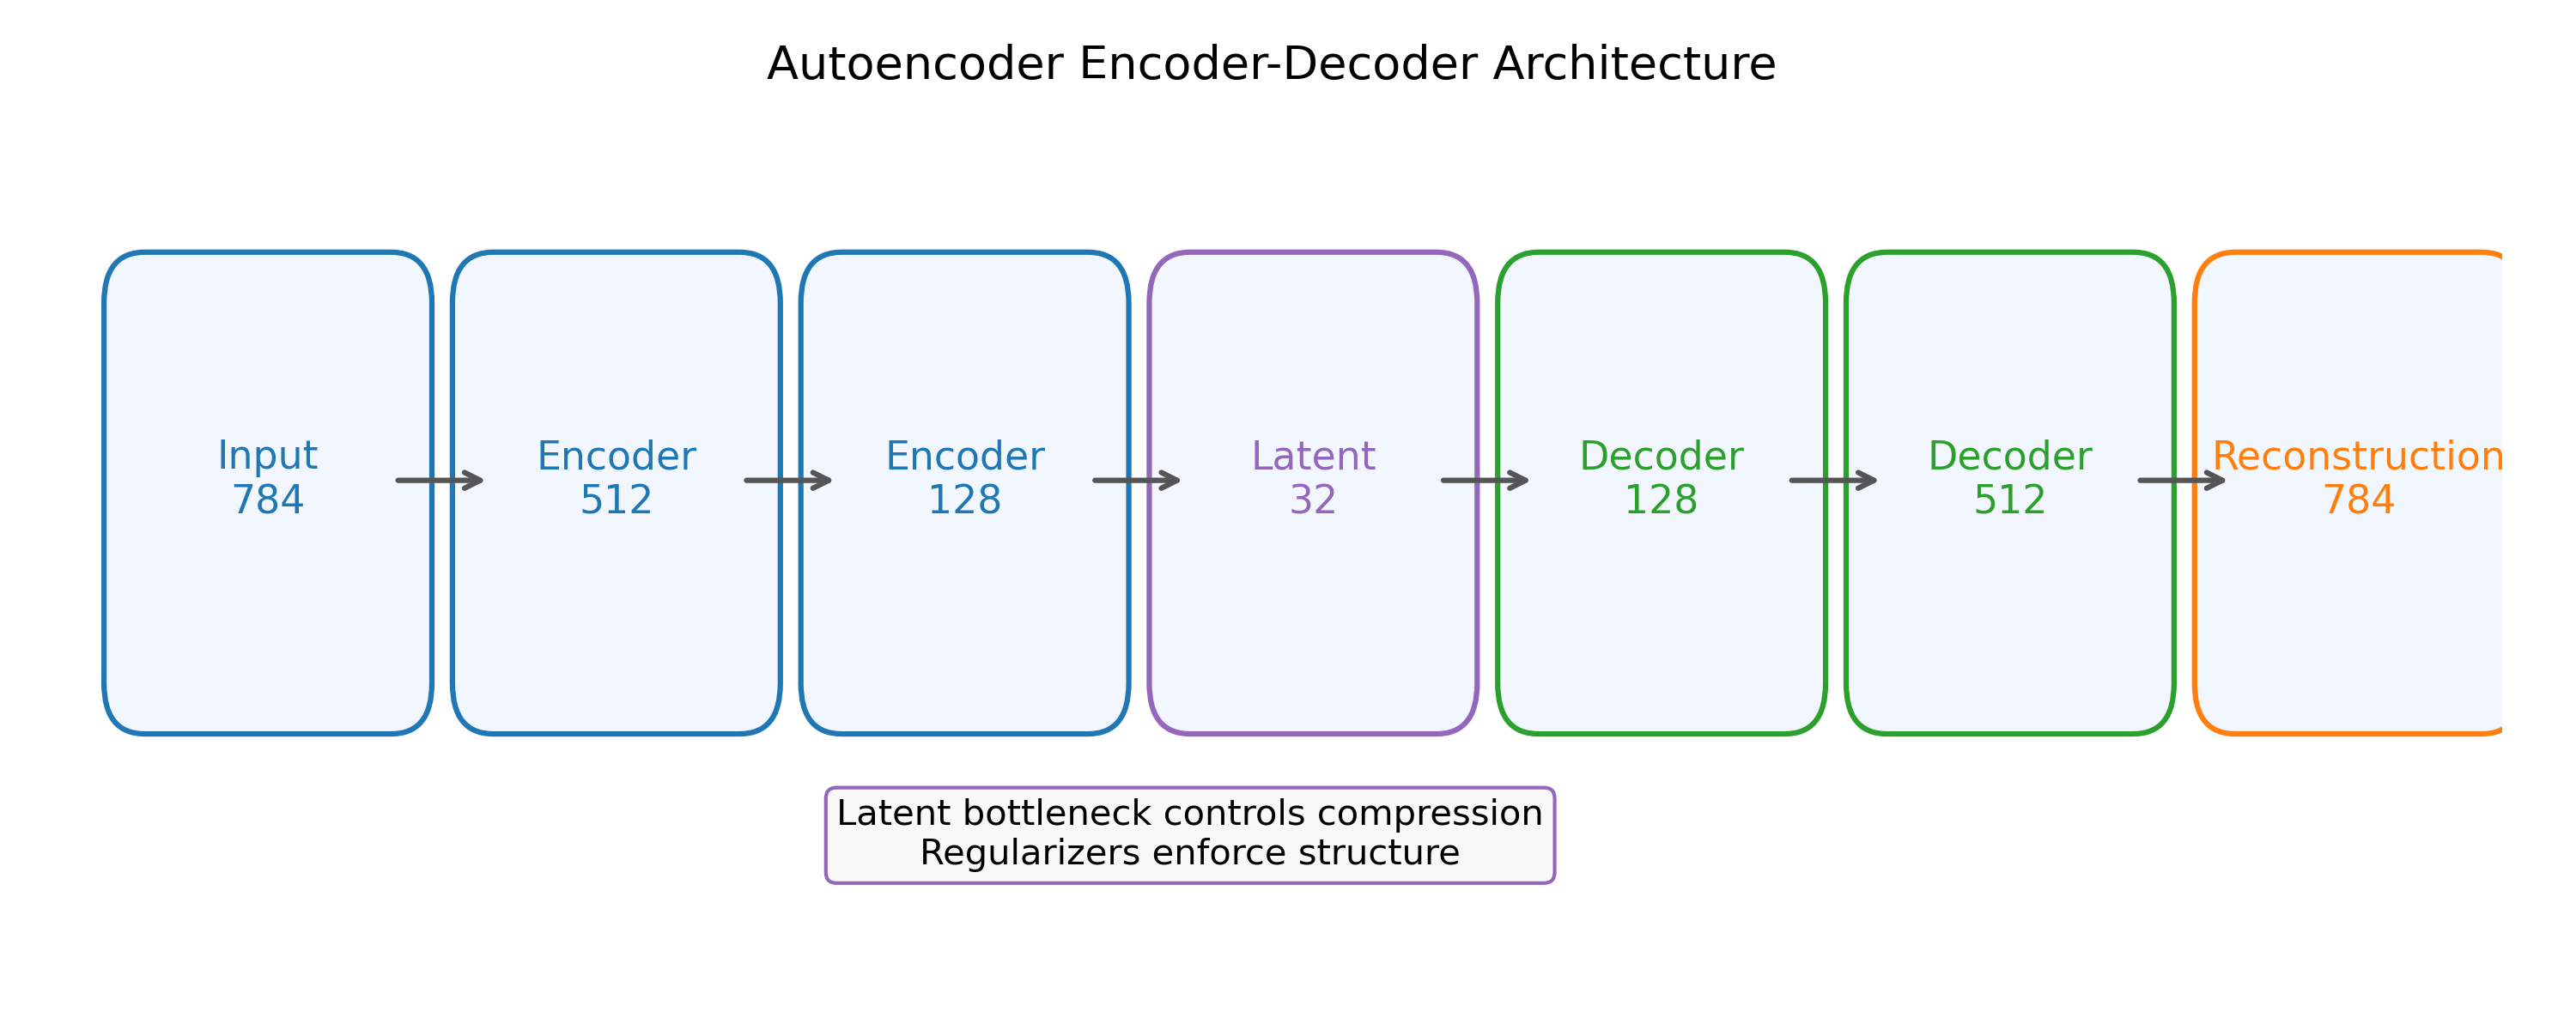
\includegraphics[width=0.8\textwidth]{autoencoder_architecture.png}
  \caption{自编码器结构,瓶颈维度决定压缩率。}
  \label{fig:autoencoder_architecture_cn}
\end{figure}

\begin{figure}[H]
  \centering
  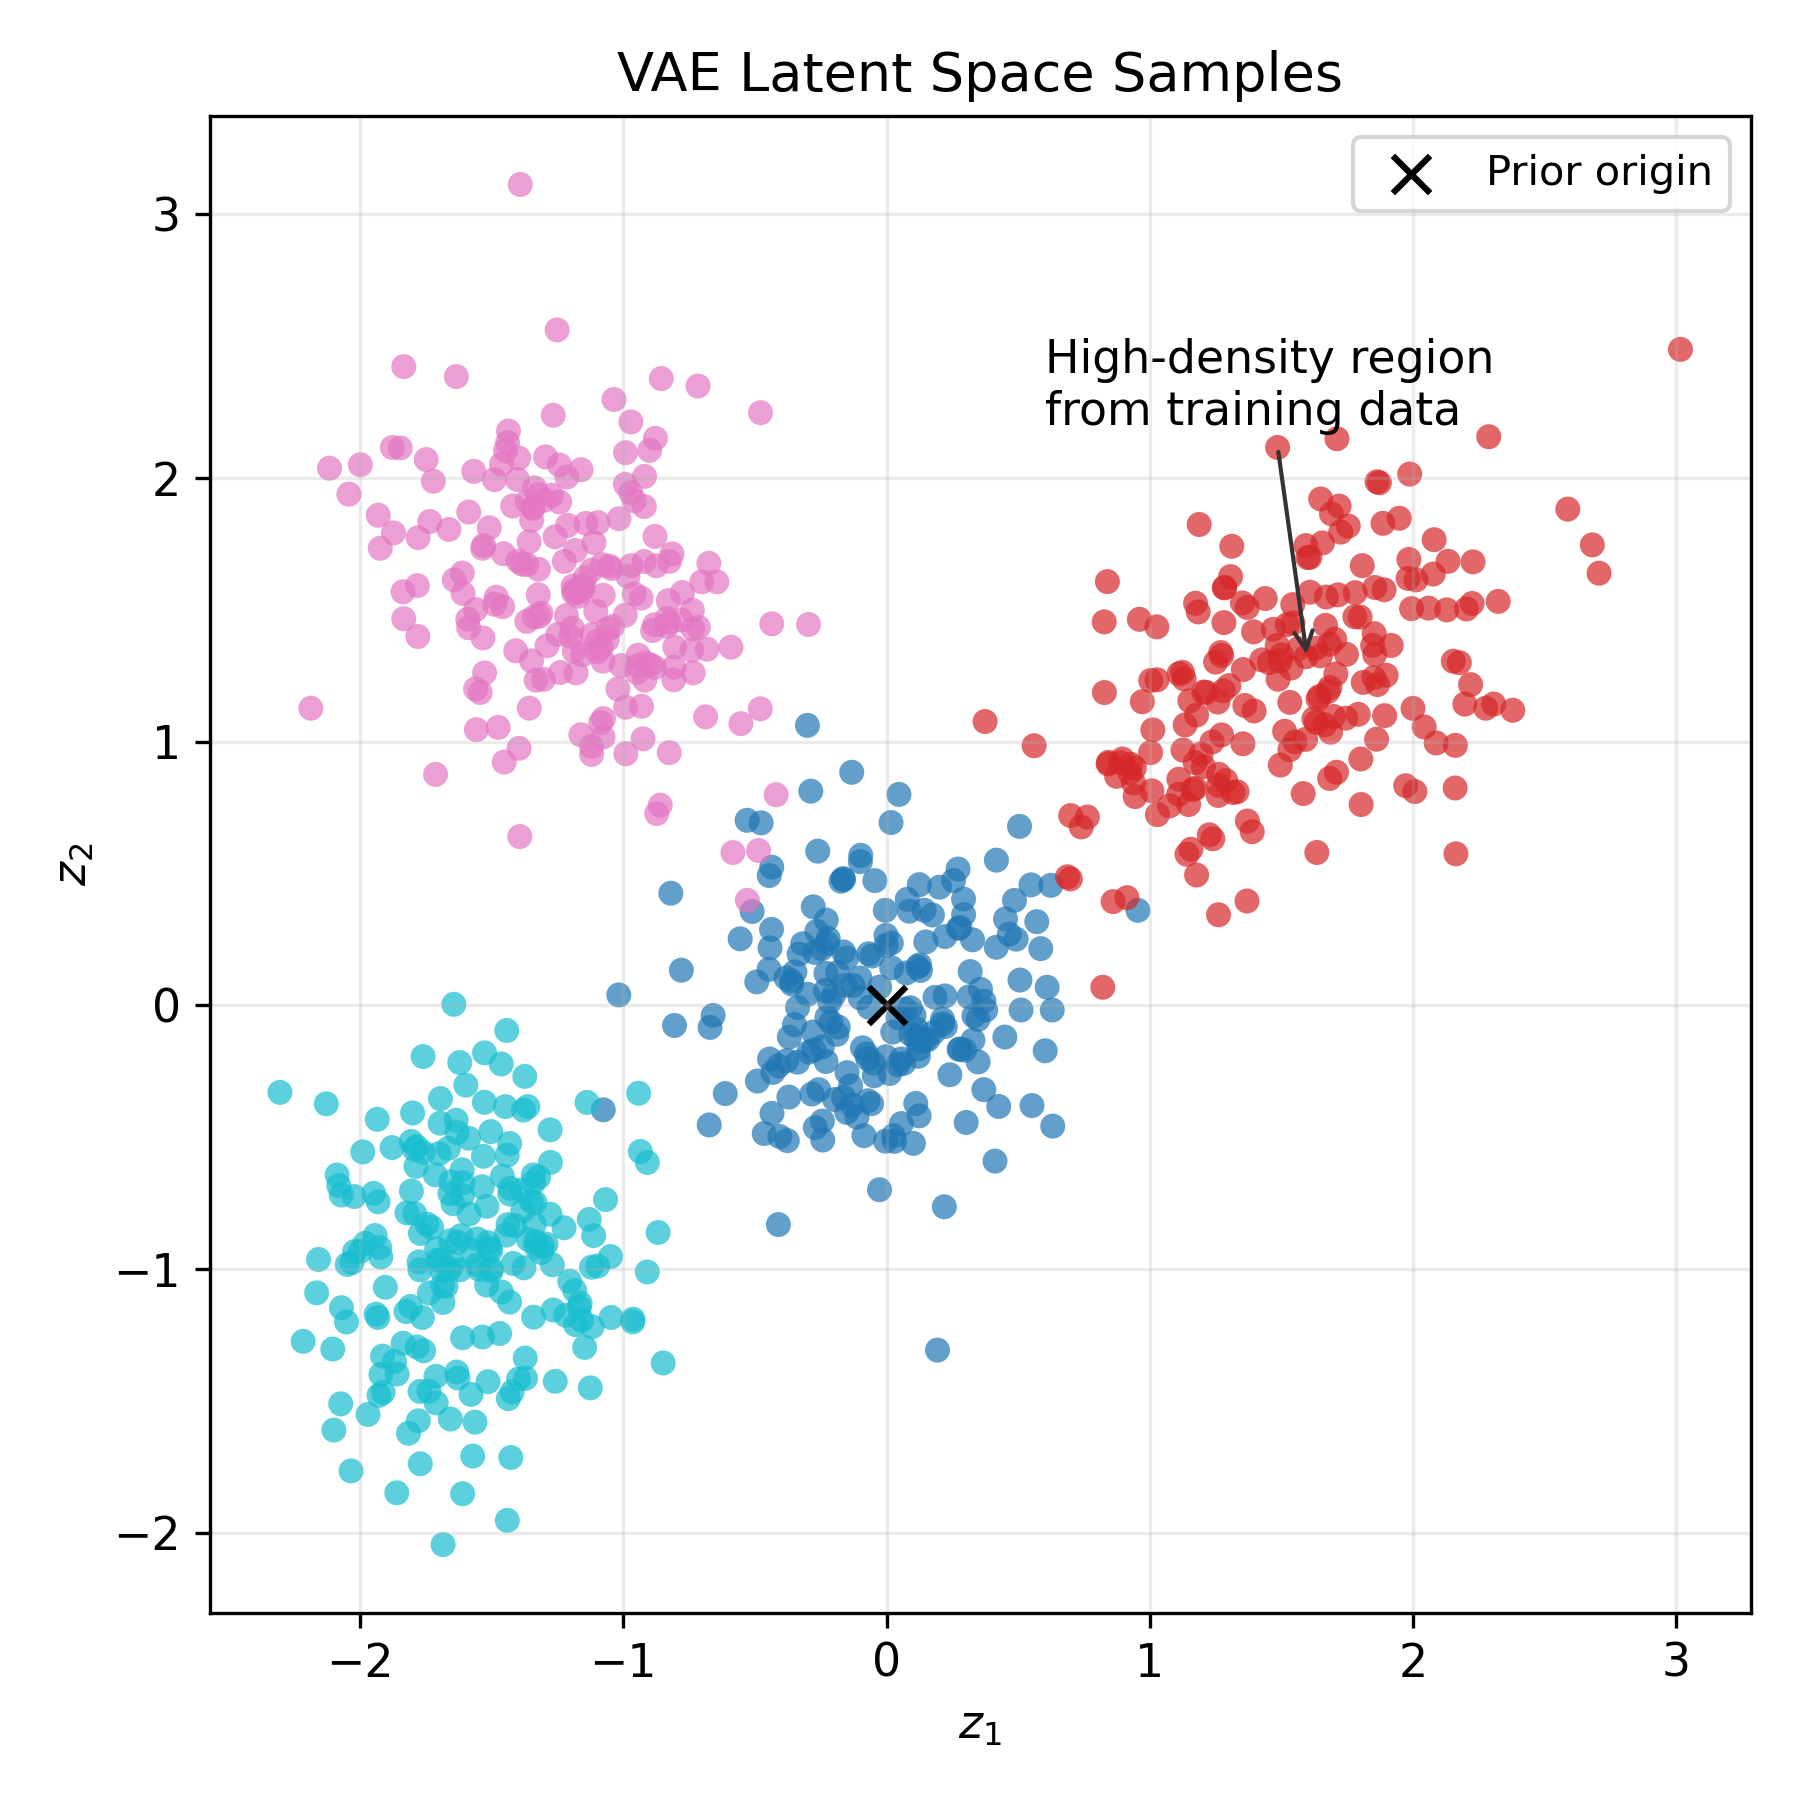
\includegraphics[width=0.8\textwidth]{vae_latent_space.png}
  \caption{VAE 潜空间采样示意,靠近原点的样本更可能生成高质量重建。}
  \label{fig:vae_latent_space_cn}
\end{figure}
\FloatBarrier

\section{生成对抗网络(GAN, DCGAN, WGAN, StyleGAN)}
GAN 通过生成器 $G$ 与判别器 $D$ 的对抗博弈学习数据分布。经典目标函数为
\begin{equation}
  \min_{G} \max_{D} \; \mathbb{E}_{\mathbf{x} \sim p_{\mathrm{data}}}[\log D(\mathbf{x})] + \mathbb{E}_{\mathbf{z} \sim p(\mathbf{z})}[\log (1 - D(G(\mathbf{z})))],
\end{equation}
驱使 $G$ 生成逼真样本。图~\ref{fig:gan_training_dynamics_cn} 展示了典型训练动态与模式覆盖。

\subsection{主要变种}
\begin{itemize}
  \item \textbf{DCGAN:} 使用卷积+反卷积架构,配合 BatchNorm、Leaky ReLU 增强图像生成稳定性。
  \item \textbf{WGAN / WGAN-GP:} 将目标替换为地球移动距离:
  \begin{equation}
    \min_{G} \max_{D \in \mathcal{D}_1} \; \mathbb{E}_{\mathbf{x} \sim p_{\mathrm{data}}}[D(\mathbf{x})] - \mathbb{E}_{\mathbf{z} \sim p(\mathbf{z})}[D(G(\mathbf{z}))],
  \end{equation}
  并通过梯度惩罚 $\lambda (\|\nabla_{\hat{\mathbf{x}}} D(\hat{\mathbf{x}})\|_2 - 1)^2$ 保持 1-Lipschitz。
  \item \textbf{StyleGAN:} 引入风格化调制,使用映射网络将潜变量 $\mathbf{z}$ 映射到 $\mathbf{w}$,通过自适应实例归一化控制多尺度特征;路径长度正则与噪声注入提升质量。
\end{itemize}

\subsection{稳定训练技巧}
GAN 易遇到模式崩塌、梯度消失等问题,可采用以下策略:
\begin{itemize}
  \item 特征匹配、minibatch discrimination 对生成器施加额外约束。
  \item 谱归一化通过缩放权重矩阵实现 Lipschitz 约束。
  \item 双时间尺度更新(TTUR)为判别器与生成器设定不同学习率,避免失衡。
\end{itemize}

\subsection{评估指标}
Fréchet Inception Distance (FID) 近似衡量真实与生成分布的 Wasserstein-2 距离:
\begin{equation}
  \mathrm{FID} = \|\boldsymbol{\mu}_r - \boldsymbol{\mu}_g\|_2^2 + \mathrm{Tr}\left(\boldsymbol{\Sigma}_r + \boldsymbol{\Sigma}_g - 2(\boldsymbol{\Sigma}_r \boldsymbol{\Sigma}_g)^{1/2}\right).
\end{equation}
还可结合精确率/召回率、Inception Score 进行综合评估。

\subsection{StyleGAN2 生成器前向示例}
\begin{lstlisting}[language=Python, caption={简化版 StyleGAN2 生成块,展示风格调制。}]
class StyledConv(nn.Module):
    def __init__(self, in_channels, out_channels, style_dim, upsample):
        super().__init__()
        self.upsample = upsample
        self.weight = nn.Parameter(torch.randn(1, out_channels, in_channels, 3, 3))
        self.modulation = nn.Linear(style_dim, in_channels)
        self.noise_weight = nn.Parameter(torch.zeros(1, out_channels, 1, 1))
        self.activation = nn.LeakyReLU(0.2)

    def forward(self, x, style, noise):
        style = self.modulation(style).view(-1, 1, x.size(1), 1, 1)
        weight = self.weight * (style + 1e-8)
        if self.upsample:
            x = upsample_2x(x)
        x = conv2d_modulated(x, weight)
        x = x + self.noise_weight * noise
        return self.activation(x)
\end{lstlisting}

\begin{figure}[H]
  \centering
  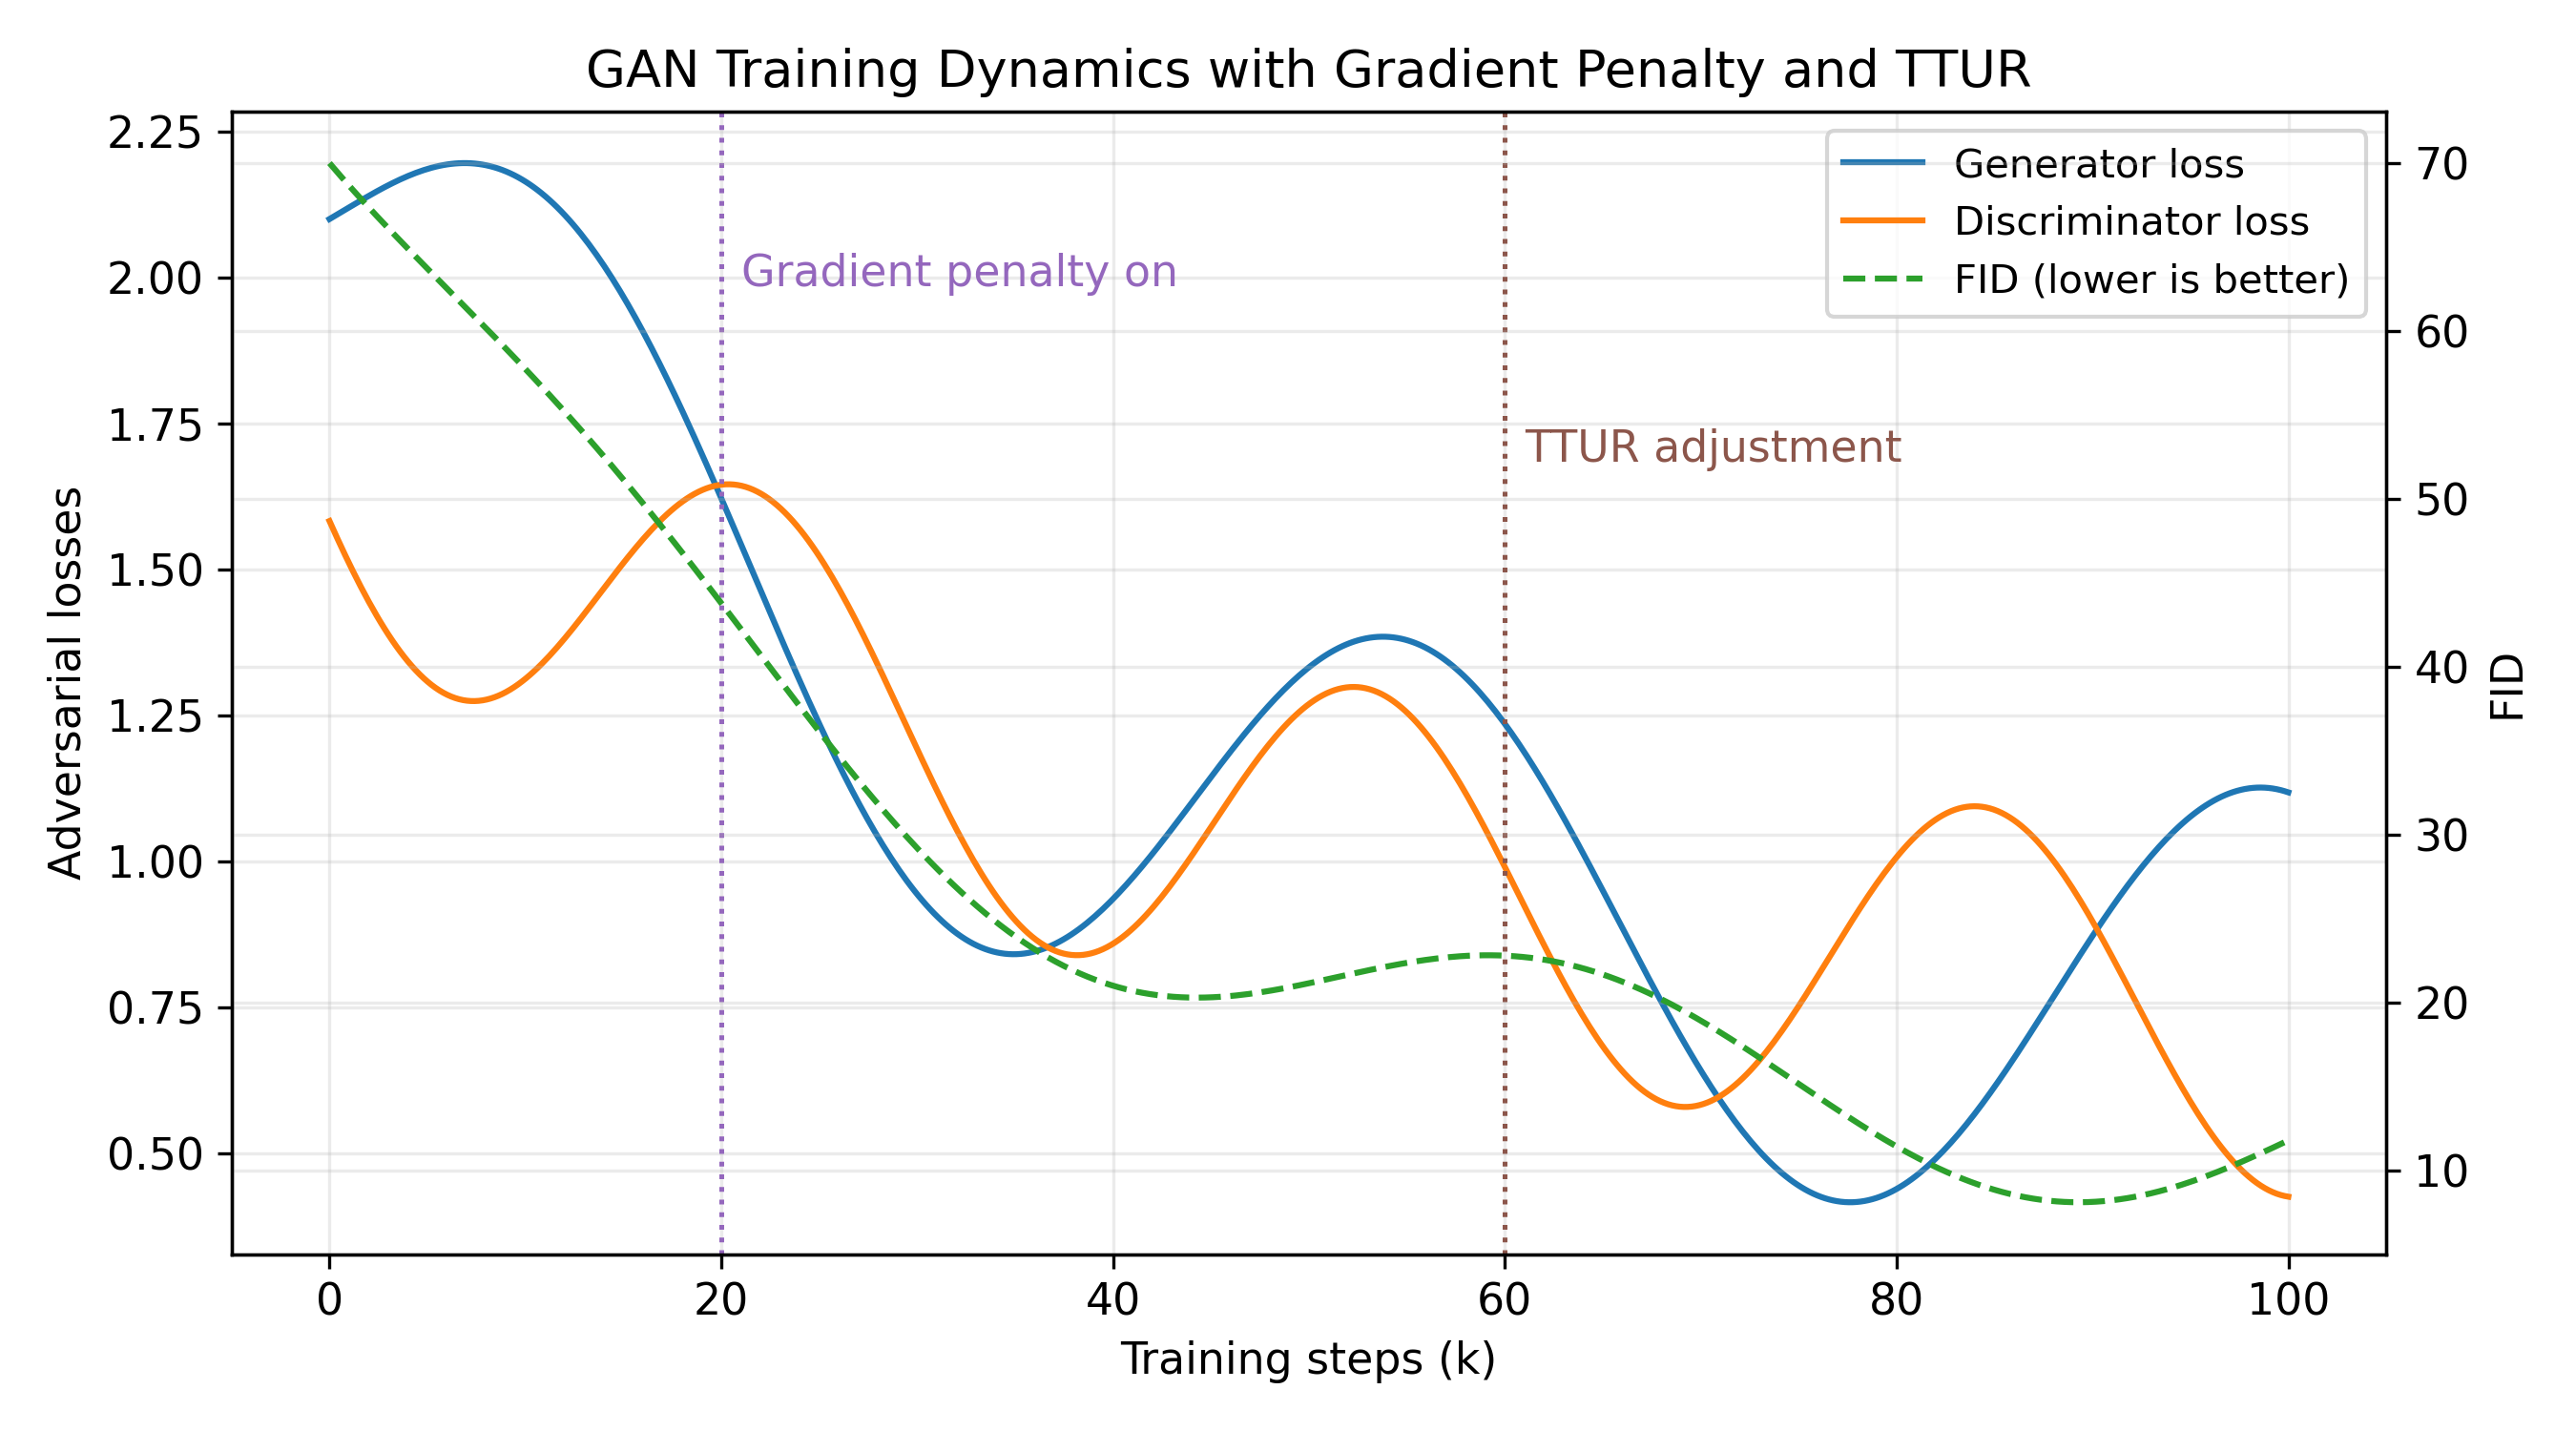
\includegraphics[width=0.85\textwidth]{gan_training_dynamics.png}
  \caption{加入梯度惩罚与 TTUR 后的 GAN 训练损失曲线。}
  \label{fig:gan_training_dynamics_cn}
\end{figure}
\FloatBarrier

\section{Diffusion Model 简介}
扩散模型通过逆转逐步加噪过程生成数据。前向过程将 $\mathbf{x}_0$ 转化为噪声 $\mathbf{x}_T$,使用方差序列 $\{\beta_t\}_{t=1}^{T}$:
\begin{equation}
  q(\mathbf{x}_t \mid \mathbf{x}_{t-1}) = \mathcal{N}\bigl(\sqrt{1 - \beta_t}\,\mathbf{x}_{t-1}, \beta_t \mathbf{I}\bigr).
\end{equation}
由于高斯可组合,有
\begin{equation}
  q(\mathbf{x}_t \mid \mathbf{x}_0) = \mathcal{N}\bigl(\sqrt{\bar{\alpha}_t}\,\mathbf{x}_0, (1 - \bar{\alpha}_t)\mathbf{I}\bigr), \quad \bar{\alpha}_t = \prod_{s=1}^{t} (1 - \beta_s).
\end{equation}

\subsection{DDPM}
模型学习噪声预测器 $\epsilon_\theta(\mathbf{x}_t, t)$,简化训练目标为
\begin{equation}
  \mathcal{L}_{\mathrm{simple}} = \mathbb{E}_{t, \mathbf{x}_0, \boldsymbol{\epsilon}} \left[ \|\boldsymbol{\epsilon} - \epsilon_\theta(\sqrt{\bar{\alpha}_t}\mathbf{x}_0 + \sqrt{1 - \bar{\alpha}_t}\,\boldsymbol{\epsilon}, t)\|_2^2 \right].
\end{equation}
采样从 $\mathbf{x}_T \sim \mathcal{N}(\mathbf{0}, \mathbf{I})$ 开始,逐步去噪:
\begin{equation}
  \mathbf{x}_{t-1} = \frac{1}{\sqrt{1 - \beta_t}} \left( \mathbf{x}_t - \frac{\beta_t}{\sqrt{1 - \bar{\alpha}_t}} \epsilon_\theta(\mathbf{x}_t, t) \right) + \sigma_t \mathbf{z}, \quad \mathbf{z} \sim \mathcal{N}(\mathbf{0}, \mathbf{I}).
\end{equation}
图~\ref{fig:diffusion_process_cn} 展示了正向与反向过程。

\subsection{改进与变体}
\begin{itemize}
  \item \textbf{引导式扩散:} 通过分类器梯度调整噪声预测 $\hat{\epsilon} = \epsilon_\theta - \sigma_t \nabla_{\mathbf{x}_t} \log p_\phi(y \mid \mathbf{x}_t)$,提升条件生成质量。
  \item \textbf{基于分数的模型:} 直接学习 $\nabla_{\mathbf{x}} \log q_t(\mathbf{x})$,使用随机微分方程与预测—校正采样器。
  \item \textbf{潜空间扩散:} 先用 VAE 压缩为潜空间再做扩散(如 Stable Diffusion),大幅降低计算量,并利用跨注意力实现多模态条件。
\end{itemize}

\subsection{伪代码}
\begin{lstlisting}[language=Python, caption={采用余弦噪声调度的扩散训练步骤。}]
def diffusion_training_step(model, scheduler, x0):
    t = torch.randint(0, scheduler.num_steps, (x0.size(0),), device=x0.device)
    noise = torch.randn_like(x0)
    alpha_bar = scheduler.alpha_bar(t).view(-1, 1, 1, 1)
    xt = torch.sqrt(alpha_bar) * x0 + torch.sqrt(1 - alpha_bar) * noise
    noise_pred = model(xt, t)
    loss = (noise - noise_pred).pow(2).mean()
    loss.backward()
    optimizer.step()
    optimizer.zero_grad()
    return loss
\end{lstlisting}

\begin{figure}[H]
  \centering
  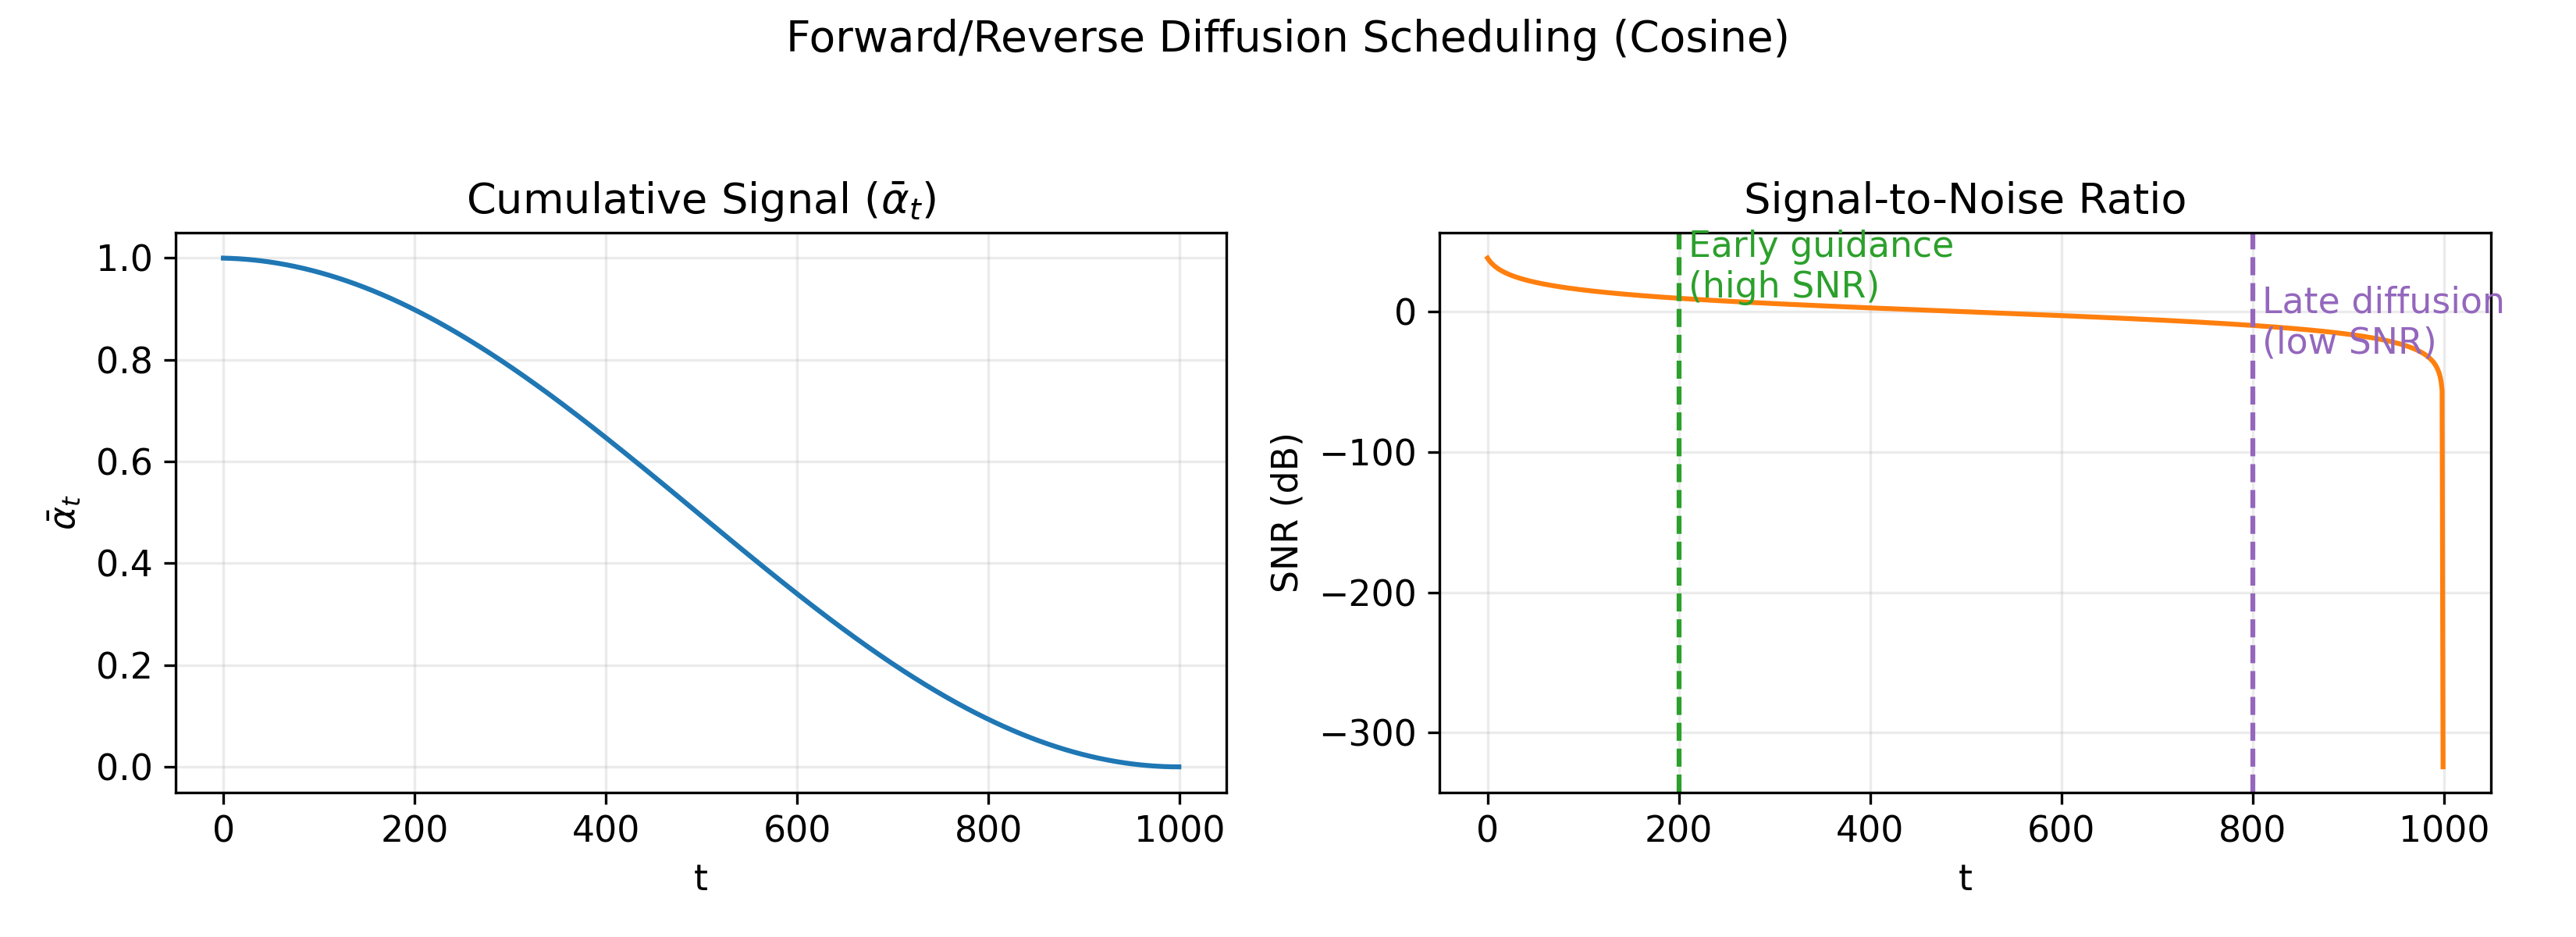
\includegraphics[width=0.85\textwidth]{diffusion_process.png}
  \caption{扩散模型的加噪与去噪轨迹,可视化余弦调度下的信噪比变化。}
  \label{fig:diffusion_process_cn}
\end{figure}
\FloatBarrier

\section*{延伸阅读}
\begin{itemize}
  \item Diederik P. Kingma \& Max Welling:《Auto-Encoding Variational Bayes》,ICLR 2014。
  \item Ian Goodfellow 等:《Generative Adversarial Networks》,NIPS 2014。
  \item Tero Karras 等:《Analyzing and Improving the Image Quality of StyleGAN》,CVPR 2020。
  \item Jonathan Ho 等:《Denoising Diffusion Probabilistic Models》,NeurIPS 2020。
  \item Prafulla Dhariwal \& Alexander Nichol:《Diffusion Models Beat GANs on Image Synthesis》,NeurIPS 2021。
\end{itemize}

\end{document}
